\begin{center}
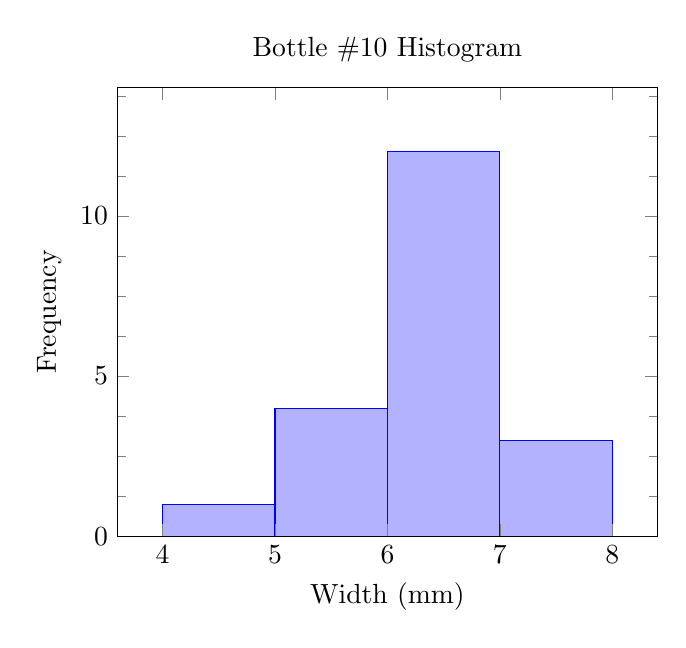
\begin{tikzpicture}
\begin{axis}[
    title={Bottle \(\#10\) Histogram},
    xlabel={Width (mm)},
    ylabel={Frequency},
    ymin=0, ymax=14,
    minor y tick num = 3,
    xtick=data,
    area style,
    ]
\addplot+[ybar interval,mark=no] plot coordinates { (4, 1) (5, 4) (6, 12) (7, 3) (8, 3) };
\end{axis}
\end{tikzpicture}
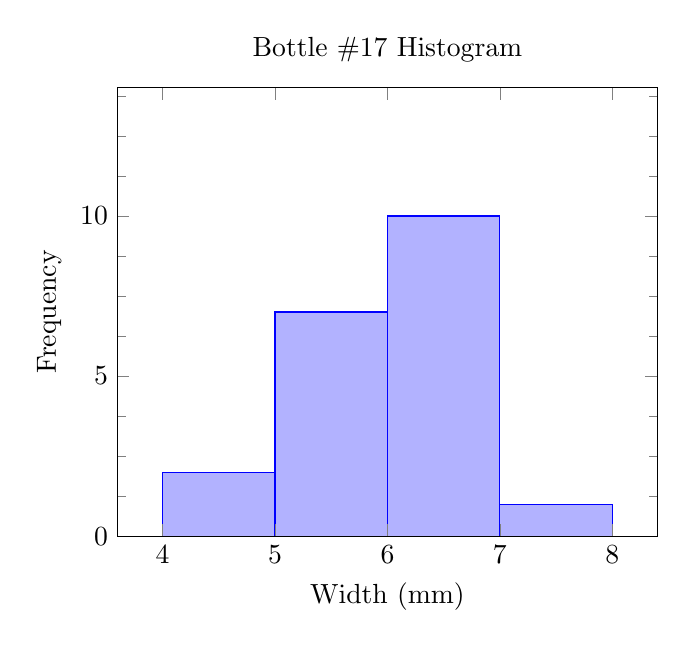
\begin{tikzpicture}
\begin{axis}[
    title={Bottle \(\#17\) Histogram},
    xlabel={Width (mm)},
    ylabel={Frequency},
    ymin=0, ymax=14,
    minor y tick num = 3,
    xtick=data,
    area style,
    ]
\addplot+[ybar interval,mark=no] plot coordinates { (4, 2) (5, 7) (6, 10) (7, 1) (8, 1) };
\end{axis}
\end{tikzpicture}
\end{center}